    % !TEX root = ../Thesis.tex
% !TEX output_directory
\documentclass[11pt,a4paper,english,greek,twoside]{../Thesis}
%\usepackage{subfig}
%\usepackage{subcaption} 
%\usepackage[demo]{graphicx}
%\usepackage{caption}
% \renewcommand\paragraph{\@startsection{paragraph}{4}{\z@}%
%                                     {-3.25ex \@plus1ex \@minus.2ex}% original: without the minus
%                                     {1.5ex plus .2ex}% original {-1em}%
%                                     {\normalfont\normalsize\bfseries}}
\begin{document}
\chapter{Ηλεκτροεγκεφαλογραφία}
\section{Βιοηλεκτρικά Σήματα και Ηλεκτροεγκεφαλογράφημα}
%Στο εισαγωγικό κεφάλαιο εστιάσαμε στην σημασία της μελέτης του εγκεφάλου και των σημάτων που μπορούμε να εξάγουμε από αυτόν.
Τα βιοηλεκτρικά σήματα είναι το αποτέλεσμα των ηλεκτροχημικών μεταβολών που λαμβάνουν χώρα εντός και μεταξύ των κυττάρων των νεύρων καθώς και των μυών. Πιο συγκεκριμένα, εάν ένα τέτοιο κύτταρο δεχθεί ερέθισμα ισχυρότερο από ένα κατώφλι συνήθως μεταξύ  -55mV και -50mV, τότε θα παράγει ένα δυναμικό δράσης το οποίο θα μεταδοθεί και θα διεγείρει γειτονικά κύτταρα. Αυτή η ομαδική δραστηριότητα των κυττάρων παράγει ηλεκτρικά πεδία ικανά να ανιχνευτούν με την βοήθεια ηλεκτροδίων τα οποία τοποθετούνται στην επιφάνεια του αντίστοιχου οργάνου, είτε στην δερματική επιφάνεια πάνω αυτό το όργανο. Όταν το ζωτικό αυτό όργανο είναι ο εγκέφαλος τότε το βιοηλεκτρικό σήμα ονομάζεται Ηλεκτροεγκεφαλογράφημα (ΗΕΓ – EEG) και η πρώτη καταγραφή ΗΕΓ, έγινε το 1924 από τον Γερμανό ψυχίατρο Hans Berger. 

Η Ηλεκτροεγκεφαλογραφία, είναι η πρώτη μέθοδος που χρησιμοποιήθηκε για την απεικόνιση της εγκεφαλικής δραστηριότητας, πριν την εμφάνιση μεθόδων όπως η μαγνητική τομογραφία (MRI) και τομογραφία εκπομπής ποζιτρονίων (PET). Παρουσιάζει σημαντικά πλεονεκτήματα όπως το ότι είναι πολύ οικονομικά προσιτή μέθοδος, συγκρινόμενη με τις άλλες που αναφέρθηκαν, και το γεγονός πως έχει πολύ χρονική ανάλυση (temporal resolution), καθώς ενώ οι μεταβολές δυναμικού του εγκεφάλου συμβαίνουν σε πολύ μικρά χρονικά διαστήματα, οι εγκεφαλογράφοι πλέον κάνουν δειγματοληψία του σήματος με συχνότητες έως και $2048Hz$, διατηρώντας σχεδόν όλη την πληροφορία του σήματος. Ωστόσο, όσον αφορά την χωρική ανάλυση (spatial resolution), ισχύει κάτι αντίστοιχο. Τα ηλεκτρικά σήματα από την στιγμή που ξεκινάνε από την πηγή τους, μέχρι να καταλήξουν στα ηλεκτρόδια, διασκορπίζονται κατά την διέλευση τους από το κρανίο. Συνεπώς το σήμα που ανιχνεύεται από ένα ηλεκτρόδιο σε μια συγκεκριμένη περιοχή δεν προέρχεται μόνο από το σημείο του εγκεφάλου που καλύπτει, αλλά και από τα γειτονικά. Αυτό το πρόβλημα μπορεί να αντιμετωπιστεί κάνοντας χρήση περισσότερων ηλεκτροδίων, και χρήσης τεχνικών χωρικού φιλτραρίσματος, για την λύση του αντίστροφου προβλήματος, δηλαδή την εύρεση του πραγματικού ηλεκτρικού σήματος που ξεκίνησε από κάθε περιοχή του εγκεφάλου. Ένας άλλος τρόπος είναι να χρησιμοποιηθούν ηλεκτρόδια που εισχωρούν σε μεγαλύτερο βάθος, πλησιάζοντας την πηγή του σήματος, πριν αυτό αλλοιωθεί από το κρανίο, προσφέροντας πολύ καλύτερη χωρική ανάλυση. Το εγκεφαλογράφημα που κάνει χρήση τέτοιου τύπου ηλεκτρόδια, ονομάζεται επεμβάτικο (invasive EEG).
\section{Εγκεφαλογράφος}
Η συσκευή που χρησιμοποιείται για την καταγραφή του εγκεφαλογραφήματος, ονομάζεται εγκεφαλογράφος, και είναι μια πολύπλοκη συσκευή με διάφορα υποσυστήματα. Από τις αρχές του 20ου αιώνα που δημιουργήθηκε ο πρώτος εγκεφαλογράφος, μέχρι σήμερα, έχουν υπάρξει δραματικές αλλαγές στον τρόπο υλοποίησης τους, με ποιο σημαντική την εισαγωγή της ψηφιακής τεχνολογίας στην αλυσίδα επεξεργασίας του σήματος. Τα υποσυστήματα που παραθέτονται στην συνέχεια, περιέχονται σε όλους τους σύγχρονους εγκεφαλογράφους, χωρίς να σημαίνει πως δεν υπάρχουν παραλλαγές και επιπλέον υποσυστήματα σε άλλους.

\subsection{Ηλεκτρόδια}
  Tα ηλεκτρόδια στην πραγματικότητα, είναι μετατροπείς, οι οποίοι ανιχνεύουν την κατανομή των ιόντων στην επιφάνεια των ιστών που καλύπτουν, μετατρέποντας το ιοντικό ρεύμα σε ρεύμα ηλεκτρόνιων. Τα ηλεκτρόδια χωρίζονται σε δύο βασικές κατηγορίες, τα 'υγρά' (wet) και τα 'στεγνά' (dry) και καθένα από αυτά μπορεί να είναι είτε μιας χρήσης, είτε επαναχρησιμοποιούμενο. 
\begin{itemize}
    \item{Υγρά (Wet) Ηλεκτρόδια}
    \par Σε αυτόν τον τύπο, χρησιμοποιείται αγώγιμο υγρό μεταξύ του δέρματος και του ηλεκτροδίου προκειμένου να επιτευχθεί αντίσταση επαφής περίπου $5kΩ$ \cite{}, έτσι ώστε να εξασφαλιστεί καλή ποιότητα σήματος ΗΕΓ με υψηλό λόγο σήματος προς θόρυβο (SNR). Ο συχνότερος τύπος ‘υγρών’ ηλεκτροδίων είναι τα αργύρου-χλωριούχου αργύρου (Ag – AgCL), τα οποία αποτελούνται απο ένα δισκίο, από καθαρό άργυρο $99.9\% $, επικαλυμένα από ένα λεπτό στρώμα χλωριούχου αργύρου. Είναι ευρέως χρησιμοποιούμενα λόγω του χαμηλού κόστους τους, της ευκολίας στην χρήση τους, καθώς και το ότι δεν είναι τοξικά. σε μορφή δισκίων η κυπέλλων \textcolor{red}{(βαλε εικονα)}.  
    \par Ένα άλλο είδος υγρών ηλεκτροδίων, χρησιμοποιούνται στον εγκεφαλογράφο Epoc που κατασκευάζεται από την εταιρεία Emotiv, και αποτελούνται από ένα χάλκινο ηλεκτρόδιο, επικαλυμμένο από μια λεπτή στρώση χρυσού. Η επαφή με το δέρμα γίνεται μέσω ενός κυλινδρικού σφουγγαριού (felt pad), το οποίο διαποτίζετε σε αλατούχο διάλυμα (saline) για την ελάττωση της αντίστασης επαφής.
    \par Παρότι η επίδοση των υγρών ηλεκτροδίων είναι πολύ ικανοποιητική, και χρησιμοποιείται ως σημείο αναφοράς για τις νέες τεχνολογίες ηλεκτροδίων που εμφανίζονται, μια σειρά απο μειονεκτήματα, εμποδίζει την χρήση τους σε περιβάλλοντα εκτός εργαστηρίου. Το πρώτο και βασικότερο είναι η δυσκολία που έχουν στην εφαρμογή τους και η άβολη αίσθηση που έχουν κατά την χρήση τους λόγω του υγρού στοιχείου. Συνήθως, απαιτείται ειδικός καθαρισμός  του σημείου επαφής πριν την χρήση, για την επίτευξη καλύτερου σήματος, αλλά και μετά το πέρας της διαδικασίας, για να καθαριστεί το δέρμα από  τα υπολείμματα του αγώγιμου υγρού. Επιπλέον, η επίτευξη της επιθυμητής αντίστασης που αναφέρθηκε προηγουμένως, μπορεί να καθυστερήσει σημαντικά. Τέλος, λόγω της πτητικότητας του αγώγιμου υγρού, υπάρχει ένα μικρό περιθώριο λίγων ωρών, πριν να ξαναχρειαστεί να το ανανεώσουμε.
    
    \item{Στεγνά (Dry) Ηλεκτρόδια}
    \par Τα προηγούμενα μειονεκτήματα έρχεται να τα καλύψει μια νέα τεχνολογία ηλεκτροδίων που δεν χρησιμοποιούν κάποιο αγώγιμο υγρό, αλλά εκμεταλλεύομενα τις εξελίξεις στον τομέα τεχνολογίας υλικών και των μικρο-συστημάτων (MEMS), προσπαθούν να επιτύχουν ποιότητα σήματος συγκρίσιμη με αυτή των υγρών ηλεκτροδίων. Λόγω της έλειψης αγώγιμου υγρού, η αντίσταση επαφής μεταξύ των ηλεκτροδίων και του δέρματος είναι πολύ μεγαλύτερη σε σχέση με τα υγρά ηλεκτρόδια, συνεπώς περιέχουν και έναν χαμηλής ενέργειας ενισχυτή οργανολογίας (instrumental amplifier) με πολύ υψηλή αντίσταση εισόδου, προκειμένου να υπάρχει όσο το δυνατόν μικρότερη απώλεια σήματος, και γι αυτό το λόγο αναφέρονται και στην βιβλιογραφία και ως ενεργά στεγνά ηλεκτρόδια (active dry electrodes). Υπάρχουν αρκετές κατηγορίες τέτοιων ηλεκτροδίων ανάλογα με την τεχνολογία κατασκευής τους και τον τρόπο επαφής τους με το δέρμα. Τα ακιδωτά ηλεκτρόδια αποτελούνται από μια συστοιχία ακίδων που είτε έρχεται σε επαφή με το δέρμα, είτε το τρυπάει για ελάχιστα μικρόμετρα, προκειμένου να διαπεράσει την εξωτερική του στρώση (stratum corneum), η οποία και ευθύνεται για το μεγαλύτερο ποσοστό της αντίστασης επαφής μεταξύ δέρματος και ηλεκτροδίου \cite{lopez2014dry}. Στη δημοσίευση \cite{sullivan2007low} χρησιμοποίησαν πυκνωτικά ηλεκτρόδια που δεν έρχονται σε επαφή με το δέρμα, προκειμένου να αποφύγουν αλλοίωση του σήματος με τα μαλλιά, αυξάνωντας όμως δραματικά την αντίσταση μεταξύ δέρματος και ηλεκτροδίου. Παρότι η έρευνα προς αυτή του του είδους τα ηλεκτρόδια φαίνεται ελπιδοφόρα και ικανή να αντιμετωπίσει τα προβήματα των υγρών ηλεκτροδίων, στην πλειοψηφία των δημοσιέυσεων είτε δεν αναφέρονται λεπτομέρειες σχετικά με την κατασκευή τους, είτε δεν γίνεται σύγκριση των αποτελεσμάτων με τις επιδόσεις των υγρών ηλεκτροδίων, συνεπώς υπάρχει ακόμα δρόμος προς αυτήν την κατεύθυνση \cite{lopez2014dry}.
    

\end{itemize}
\subsection{Ενίσχυση και Επεξεργασία Σημάτων}
  Τα σήματα που λαμβάνονται από τα ηλεκτρόδια στην επιφάνεια του δέρματος κυμαίνονται μεταξύ $10μV$ και $100μV$, και πρέπει να ενισχυθούν σημαντικά προκειμένου να γίνει η επεξεργασία τους στα επόμενα στάδια. Το στάδιο της ενίσχυσης περιλαμβάνει αρχικά έναν διαφορικό ενισχυτή με υψηλή απόρριψη κοινού σήματος, και στη συνέχεια δύο η τρία ξεχωριστά στάδια ενίσχυσής με μεγάλο κέρδος. Επειδή τα σήματα αυτά περιέχουν πολύ θόρυβο σε συχνότητες κοντά στα $0Hz$ (DC συνιστώσα), καθώς και στα $50Hz$ η $60Hz$, λόγω των ηλεκτρομαγνητικών παρεμβολών από ρεύματα τροφοδοσίας στον χώρο. Συνεπώς το σήμα πρέπει να περάσει από διάφορα στάδια υψιπερατού και βαθυπερατού φιλτραρίσματος. Τέλος προκειμένου να σταλθούν τα σήματα στο επόμενο στάδιο της αποθήκευσης και απεικόνισης, γίνεται η χρήση ενός Digital to Analog Converter (DAC). Εδώ φαίνεται και μια από τις χρησιμότητες της ενίσχυσης, καθώς τα DAC δεν μπορούν να λειτουργήσουν με σήματα εισόδου της τάξης των $μVolt$. Τέλος μετά την ψηφιοποίηση του σήματος χρησιμοποιούνται οπτικοί απομονοτές (optical isolator) για λόγους ασφαλείας, έτσι ώστε να μην υπάρχει κίνδυνος να διαρέυσει ρεύμα από τα επόμενα στάδια (π.χ υπολογιστής), προς τον χρήστη του εγκεφαλογράφου.

\subsection{Μονάδα Αποθήκευσης και Απεικόνισης Σημάτων}
  Αυτό το στάδιο αποτελείται απο μια υπολογιστική μονάδα η οποία αποθηκεύει τα σήματα, και χρησιμοποιεί λογισμικό για την απεικόνιση των σημάτων. Επιπλέον σε πολλές περιπτώσεις υπάρχει η δυνατότητα χρήσης επιπλέον τεχνικών επεξεργασίας σε αυτό το στάδιο, όπως χρήση ψηφιακών φίλτρων, κατάτμηση του σήματος σε σημεία ενδιαφέροντος κ.α .

\section{Σύστημα 10-20}
Το σύστημα 10-20 χρησιμοποιείται διεθνώς για να περιγράψει και να ορίσει την θέση των ηλεκτροδίων στο κεφάλι. Η χρήση ενός τέτοιου συστήματος είναι απαραίτητη, προκειμένου να υπάρχει ένα κοινό σημείο αναφοράς μεταξύ των ερευνητών για την αναπαραγωγή και σύγκριση των διαφόρων μεθοδολογιών στην εγκεφαλογραφία.
Οι αριθμοί $'10'$ και $'20'$ είναι ποσοστά και συμβολίζουν το $10\% $ και $20\% $  της απόστασης μεταξύ των δύο αυτιών, τα οποία με την σειρά τους ορίζουν την απόσταση από ένα αυτί προς το πλησιέστερο σε αυτό ηλεκτρόδιο και την απόσταση μεταξύ δύο γειτονικών ηλεκτροδίων αντίστοιχα.

\begin{figure}[h]
  \centering
  \noindent\makebox[\textwidth]{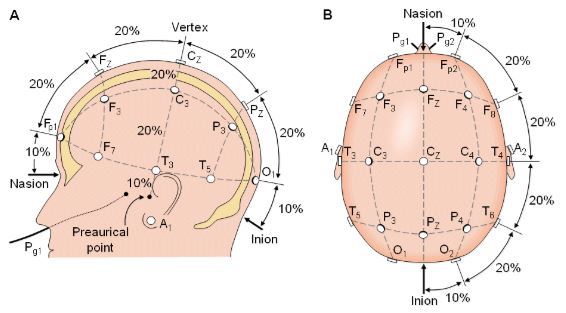
\includegraphics[scale=0.8]{{ImagesSSVEP/10_20}.jpg}}
  \captionsetup{singlelinecheck = false, justification=justified} % used for left alignment
  \caption{Τοποθεσίες ηλεκτροδίων με βάση το σύστημα 10-20.\\ Εικόνα από \cite{Malmivuo1995-jf}. }
  \label{fig:10_20}
\end{figure}

Ανάλογα με την εγκεφαλική περιοχή που καλύπτουν τα ηλεκτρόδια, παίρνουν και το όνομά τους που αποτελείται από ένα γράμμα (η συνδυασμό γραμμάτων) και έναν ζυγό αριθμό για το δεξί ημισφαίριο και περιττό για το αριστερό ημισφαίριο. Η βασική διάταξη που αποτελείται από 19 ηλεκτρόδια, είναι η εξής :

\begin{itemize}
    \item Προμετωπιαίος φλοιός (Pre-Frontal cortex) : Fp1, Fp2
    \item Μετωπιαίος λοβός (Frontal lobe) : F3, F4, F7, F8, Fz
    \item Κροταφικός λοβός (Temporal lobe) : T3, T4, T5, T6
    \item Βρεγματικός λοβός (Parietal lobe) : P3, P4, Pz
    \item Ινιακός λοβός (Occipital lobe) : O1, O2
    \item Κεντρική περιοχή (Central) : C3, C4, Cz
\end{itemize}
\par Ο δείκτης z, προσδιορίζει τα ηλεκτρόδια τα οποία βρίσκονται πάνω στην διαχωριστική γραμμή μεταξύ των δύο ημισφαιρίων.
Το παραπάνω σύστημα μπορεί να επεκταθεί έτσι ώστε να καλύψει καταστάσεις στις οποίες απαιτείται μεγαλύτερος αριθμός ηλεκτροδίων, ορίζοντας νέες εγκεφαλικές περιοχές μεταξύ αυτών που αναφέρθηκαν, ή και διαφορετικές σχετικές αποστάσεις μεταξύ των ηλεκτροδίων.
\begin{figure}[h]
  \centering
  \noindent\makebox[\textwidth]{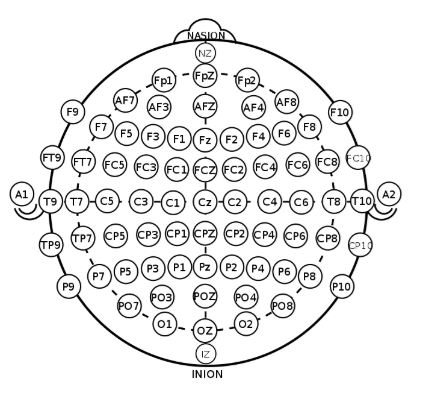
\includegraphics[scale=0.6]{{ImagesSSVEP/10_20_ext}.jpg}}
  \captionsetup{singlelinecheck = false, justification=justified} % used for left alignment
  \caption{Επέκταση συστήματος 10-20. Εικόνα από \cite{Malmivuo1995-jf}. }
  \label{fig:10_20_ext}
\end{figure}

\section{Διεπαφές εγκεφάλου – υπολογιστή (Brain Computer Interfaces)}
  \par Όπως αναφέρθηκε και στην εισαγωγική ενότητα \ref{sec:importance}, οι διεπαφές εγκεφάλου - υπολογιστή (BCIs) εκμεταλλευόμενες την εξέλιξη στις τεχνικές ανάλυσης σημάτων του εγκεφάλου, επιτρέπουν στους χρήστες να επικοινωνούν με το εξωτερικό περιβάλλον χωρίς να απαιτείται οποιαδήποτε μυική κίνηση του χρήστη, μεταφέροντας μηνύματα και εντολές από το μυαλό τους στον υπολογιστή. Στο παρελθόν, η ιδέα ενός BCI το οποίο θα αποκωδικοποιεί τις σκέψεις ενός ατόμου και θα τις μετατρέπει σε εντολές κατανοητές από έναν υπολογιστή, αντιμετωπίστηκε πολύ επιφυλακτικά, ως ένα πολύ περίπλοκο πρόβλημα, λόγω των τεχνικών περιορισμών που υπήρχαν, όπως η χαμηλή χρονική και χωρική ανάλυση καταγραφών, κόστος υλοποίησης real-time εφαρμογών. Σήμερα όμως, η χρήση τέτοιων διεπαφών έχει εξελιχθεί αρκετα και η πληθώρα των υλοποιήσεων έχει οδήγησε στην ανάγκη κατηγοριοποίησης τους. Σύμφωνα με την δημοσίευση \cite{Zander2010-ji} οι διεπαφές εγκεφάλου - υπολογιστή χωρίζονται σε τρεις μεγάλες κατηγορίες : 
  \label{sec:bci_categories}
  \subsection{Active BCIs}
  \par Σε αυτού του είδους τις διεπαφές, ο χρήστης είναι αυτός που συνειδητά προσπαθεί να ελέγξει τα εγκεφαλικά του κύματα, ανεξάρτητα από οποιαδήποτε εξωτερικά ερεθίσματα. Ίσως το πιο αντιπροσωπευτικό δείγμα της κατηγορίας είναι οι διεπαφές οι οποίες βασίζονται στην ανίχνευση κυματομορφών που σχετίζονται με την σκέψη κίνησης ενός μέλους του σώματος, και όχι την πραγματική κίνηση του, γνωστή και στην βιβλιογραφία ως Motor Imagery. Για παράδειγμα, όταν ένας χρήστης σκεφτέι πως κινεί το δεξί του χέρι, το πλάτος των εγκεφαλικών σημάτων στον κινητικό φλοιό αυξάνεται στο δεξί ημισφαίριο και ελαττώνεται στο αρίστερο, και αντίστοιχα για το αριστερό χέρι. Συνήθως για τις διεπαφές αυτής της κατηγορίας απαιτείται μεγάλος χρόνος εκπαίδευσης τόσο του χρήστη, για να ελέγχει και να απομονώνει τις σκέψεις του, όσο και του συστήματος, έτσι ώστε να καταλαβαίνει σωστά τις προθέσεις του χρήστη. 

  \subsection{Reactive BCIs}
  \par Σε αυτήν την κατηγορία ανήκουν οι διεπαφές των οποίων η έξοδος εξαρτάται από εγκεφαλική λειτουργία που προκαλείται ως αντίδραση σε μια εξωτερική διέγερση, η οποία έχει ρυθμιστεί έτσι ώστε να κωδικοποιεί την πρόθεση του χρήστη. Ο χρήστης εξαναγκάζει τα εγκεφαλικά του σήματα να παραμένουν σε μια συγκεκριμένη κατάσταση, απλά με το να παρατηρεί η να συγκεντρώνεται σε μια συγκεκριμένη εξωτερική διέγερση. Το πλεονέκτημα αυτών των διεπαφών είναι πως τα προκαλούμενα σήματα είναι παρόμοια από χρήστη σε χρήστη, και πως απαιτείται ελάχιστη η καθόλου εκπαίδευση για να λειτουργήσουν.

  \subsection{Passive BCIs}
  \par Τέλος, σε αυτού του τύπου τις διεπαφές, ο χρήστης δεν έχει άμεσο έλεγχο του αποτελέσματος καθώς δεν απαιτείται προσπάθεια απο τον χρήστη να ελέγξει τα εγκεφαλικά του σήματα. Αντί αυτού, η έξοδος του συστήματος επηρεάζεται από την νοητική κατάσταση του χρήστη, όπως για παράδειγμα τα επίπεδα προσοχής του, τα συναισθήματα του ή τα επίπεδα κόπωσης. Πολλές φορές σε αυτού του είδους τις διεπαφές η έξοδος τους γίνεται γνωστή στον χρήστη μέσω κάποιας ηχιτικής ή οπτικής ένδειξης, επηρεάζοντας εκ νέου την νοητική του κατάσταση, και δημιουργώντας ένα είδος ανάδρασης (neuro-feedback). 
  
  \par Παρότι η παραπάνω κατηγοριοποίηση δίνει μια σαφή εικόνα όλων των διαφορετικών BCIs, υπάρχουν περιπτώσεις όπου τα όρια μεταξύ των παραπάνω ορισμών δεν είναι απολύτως σαφή. Για παράδειγμα, στην περίπτωση της neuro-feedback ανάδρασης, ο χρήστης είναι πολύ πιθανόν να προσπαθήσει να αλλάξει την νοητική του κατάσταση επηρεαζόμενος από την έξοδο της διεπαφής, μετατρέποντας έτσι το είδος του BCI από passive σε active. Ακόμα όμως και στην περίπτωση των active διεπαφών, η πρόθεση του χρήστη για το τι εγκεφαλικά σήματα θα παράξει, επηρεάζεται από το αποτέλεσμα της προηγούμενης πρόθεσης του, το οποίο μπορεί να θεωρηθεί ως εξωτερική διέγερση, συνεπώς καταλήγουμε σε τύπο reactive. 

  \subsection{Κριτήρια Αξιολόγησης Απόδοσης των BCIs}
  \subsubsection{ITR}
  \subsubsection{Accuracy}
  
\section{Χαρακτηριστικά Εγκεφαλικά σήματα}
  \par Σε αυτό το σημείο θα αναφερθούμε σε κάποια βασικά εγκεφαλικά σήματα που παράγονται στον εγκέφαλο, είτε ακούσια είτε εκούσια, και τα οποία χρησιμοποιούνται για την υλοποίηση των διαφόρων τύπων BCIs που αναφέρθηκαν στην ενότητα \ref{sec:bci_categories}. Γενικά, τα EEG σήματα ταξινομούνται με κριτήριο την συχνότητά, το πλάτος, την μορφή, καθώς και την τοποθεσία στο κρανίο όπου καταγράφονται.
  
  \subsection{Εγκεφαλικοί ρυθμοί}
    \par Αυτού του είδους τα σήματα εμφανίζονται φυσιολογικά σε όλους του εγκεφάλους, ταξινομούνται με κριτήριο την συχνότητα τους, και η παρουσία τους ή η απουσία τους, βοηθάει την εξαγωγή συμπερασμάτων όσον αφορά τόσο την νοητική κατάσταση του χρήστη, όσο και την ύπαρξη κάποια νευρολογικής ασθένειας. Τα σχόλια για καθέναν από αυτούς αφορούν υγιής ενήλικες οργανισμούς, καθώς στην αντίθετη περίπτωση διαφοροποιούνται αρκετά τα πράγματα, και αυτοί οι ρυθμοί μπορούν να χρησιμοποιηθούν για την διάγνωση ασθενειών. 
    \begin{itemize}
        \item {Κύματα Δέλτα}
        \par Κύματα Δέλτα ονομάζουμε τις συχνότητες με εύρος $0.5 - 4 Hz$ και εμφανίζονται κυρίως σε νεογνά και ενήλικες κατά την διάρκεια του ύπνου (deep stage 3 of NREM), και ίσως εμπλέκονται στην διαδικασία σχηματισμού της μνήμης \cite{Maquet2001-cs}
        \item {Κύματα Θήτα}
        \par Κύματα Θήτα ονομάζονται οι κυματομορφές με εύρος συχνοτήτων $4 - 8Hz$ και σε φυσιολογικούς ενήλικες εμφανίζονται σε πολύ μικρή ποσότητα, και συχνά όταν κάποιος βρίσκεται στην κατάσταση της ονειροπόλησης (daydreaming)
        \item {Κύματα Άλφα}
        \par Τα κύματα Άλφα, τα οποία ήταν τα πρώτα κύματα που ανιχνεύτηκαν στον εγκέφαλο από τον Hans Berger \cite{Berger1933-pg}, και κυμαίνονται μεταξύ $7.5 - 12.5Hz$. Κυρίως εμφανίζονται στον οπτικό φλοιό κατά την διάρκεια της ξεκούρασης με κλειστά μάτια, όχι όμως σε κατάσταση ύπνου, όπου τότε ελαττώνονται. 
        \item {Κύματα Βήτα}
        \par Τα κύματα Βήτα ανακαλύφθηκαν και αυτά από τον Hans Berger, αμέσως μετά τα Άλφα, και η συχνότητα τους κυμαίνεται μεταξύ $12.5 - 30Hz$. Εμφανίζονται όταν το άτομο έχει ανοιχτά μάτια, και βρίσκεται σε κατάσταση συγκέντρωσης, όταν προσπαθεί να λύσει ένα πρόβλημα ή και σε καταστάσεις άγχους.
        \item{Κύματα Γάμμα}
        \par Το εύρος συχνοτήτων των κυμάτων Γάμμα είναι μεταξύ $30 - 80Hz$, και όπως και τα Βήτα, εντοπίζονται στον εγκέφαλο σε καταστάσεις έντονης εγρήγορσης \cite{Bressler1990-im}. Παρόλαυτα έχουν καταγραφεί και κατά τις φάσεις του REM ύπνου, κατά την οποία δεν υπάρχει συνείδηση και εγρήγορση στο άτομο \cite{Steriade1996-pg}.
    \end{itemize}

    \begin{figure}[H]
        \centering
        \noindent\makebox[\textwidth]{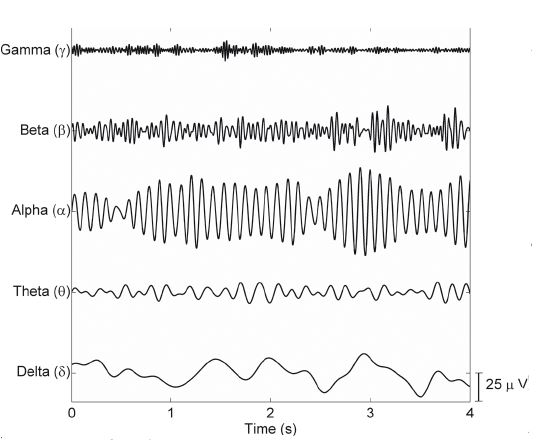
\includegraphics[scale=0.7]{{ImagesSSVEP/eeg_waves}.jpg}}
        \captionsetup{singlelinecheck = false, justification=justified} % used for left alignment
        \caption{Γραφική αναπαράσταση των φυσιολογικών κυματομορφών του εγκεφάλου. Εικόνα από \cite{Scarano2012-ok}}
        \label{fig:eeg_waves}
    \end{figure}
    %πως χρησιμοποιούνται σε BCI / efarmoges
  \subsection{Προκλητά Δυναμικά (ΠΔ)}  
    \par Ως προκλητά δυναμικά, ορίζονται οι διαφορές δυναμικού στο εγκεφαλικό σήμα που ανιχνεύονται σε συγκεκριμένο χρονικό διάστημα, ως αντίδραση σε ένα εξωτερικό ερέθισμα. Τα δυναμικά αυτά παρουσιάζουν μεγάλο ερευνητικό ενδιαφέρον και χρησιμοποιούνται κατά κόρον, τόσο για την διάγνωση ασθενειών του εγκεφάλου και των νεύρων, όσο και για την υλοποίηση BCIs.  Ένας λόγος που χρησιμοποιούνται ευρέως σε BCIs, είναι πως τα προκλητά δυναμικά μπορούν να αναπαραχθούν κατά βούληση,  κατά την διάρκεια πειραμάτων στα οποία παρέχουμε την κατάλληλη διέγερση, συνεπώς είναι πιο εύκολη η μελέτη τους για την χρήση τους σε διεπαφές εγκεφάλου - υπολογιστή, συγκριτικά με άλλα εγκεφαλικά σήματα όπως η φυσιολογικοί εγκεφαλικοί ρυθμοί, που εξαρτώνται από την ψυχολογία και την κατάσταση του ατόμου.
    Τα ΠΔ χωρίζονται σε δύο μεγάλες κατηγορίες, τα ενδογενή και τα εξωγενή δυναμικά \cite{Sutton1965-nl}.  Τα εξωγενή δυναμικά σχετίζονται άμεσα με τα χαρακτηριστικά του εξωτερικού ερεθίσματος (π.χ ένταση, συχνότητα), ενώ τα ενδογενή δυναμικά σχετίζονται με την ψυχολογική αντίδραση του ατόμου στο εξωτερικό ερέθισμα. Στη συνέχεια θα αναφερθούμε στα πιο γνωστά σήματα κάθε κατηγορίας. Τέλος αξίζει να αναφερθεί πως για κάθε μια από αυτές τις κατηγορίες, τα ερεθίσματα μπορούν να είναι διαφόρων ειδών, όπως οπτικά, ακουστικά, σωματικά κ.α.
    \subsubsection{Ενδογενή ΠΔ - P300}  
      \paragraph{Περιγραφή} ~\\
      Το ενδογενές δυναμικό που κυριαρχεί τόσο στην έρευνα όσο και στην χρήση του σε BCIs, είναι το P300 \cite{Gordeev2007-pu}. Αποτελείται από μια θετική διακύμανση στην τάση, η οποία κατά μέσο όρο προκύπτει 300ms αφότου εμφανιστεί το ερέθισμα. Το πλάτος της διακύμανσης κυμαίνεται περίπου από 30μV στην περιοχή του εγκεφάλου που καλύπτεται από το ηλεκτρόδιο Pz, ενώ αρκετά χαμηλότερο πλάτος, κοντά στα 5μV, στην περιοχή Fz \cite{Perlman2013-sg}. Προκειμένου να προκληθούν σήματα P300, το άτομο πρέπει να συγκεντρώνει την προσοχή του σε σπανίως εμφανιζόμενα ερεθίσματα (target), τοποθετημένα τυχαία ανάμεσα σε μια σειρά από συχνά εμφανιζόμενα ερεθίσματα (non target). Αυτή η διαδικασία είναι γνωστή στην ξένη βιβλιογραφία ως “oddball paradigm”. Υπάρχουν αρκετοί λόγοι που καθιστούν τα P300 τόσο δημοφιλή. Αρχικά, τα P300 είναι σήματα τα οποία μπορούν να δημιουργηθούν στον εγκέφαλο του καθενός, χωρίς να απαιτείται σχεδόν καθόλου εκπαίδευση από τον χρήστη. Επιπλέον, είναι εύκολα ανιχνεύσιμα, και αρκετά συνεπή όσον αφορά τον χρόνο που θα εμφανιστούν μετά το κατάλληλο ερέθισμα \cite{Fazel-Rezai2012-mk}. 
      
      \paragraph{Εφαρμογές} ~\\
      \par Ίσως η πιο διάσημη εφαρμογή των P300 είναι σε συστήματα BCI, και συγκεκριμένα σε μηχανές συλλαβισμού (spellers). Πρώτοι οι  Farwell και  Donchin περιέγραψαν και υλοποίησαν μια τέτοια μηχανή \cite{Farwell1988TalkingPotentials} Η διαδικασία που ακολουθήθηκε είναι η εξής. Αρχικά δημιουργήθηκε ένα γραφικό περιβάλλον, που παράγει τα οπτικά ερεθίσματα που θα προκαλέσουν τα P300, και αποτελείται από ένα πίνακα 6x6 με αλφαριθμητικούς χαρακτήρες. Κάθε γραμμή και στήλη του πίνακα, ακολουθεί ένα μοτίβο που αποτελείται από 100ms κατά τα οποία όλα τα στοιχεία της κάθε γραμμής ή στήλης έχουν υψηλή φωτεινότητα, και 80ms χαμηλή. Το μοτίβο αυτό συμβαίνει διαδοχικά σε κάθε γραμμή ή στήλη, και με τυχαία σειρά. Συνεπώς δημιουργείται μια ακολουθία 12 τέτοια μοτίβα. Ο χρήστης κάθε φορά είναι συγκεντρωμένος σε ένα συγκεκριμένο αλφαριθμητικό, το οποίο ταυτόχρονα ανήκει σε μια γραμμή και μια στήλη, που αποτελούν τα target ερεθίσματα, σε αντίθεση με τα non-target που αποτελούνται από τις άλλες 10 στήλες και γραμμές. Ανιχνεύοντας λοιπόν τα P300 σήματα που παράγονται, είναι δυνατόν να παρθεί απόφαση για το αλφαριθμητικό στο οποίο είχε συγκεντρωθεί ο χρήστης. Το ποσοστό επιτυχίας που σημείωσαν ήταν $95\%$ σε ταχύτητα 1 χαρακτήρα κάθε 26 δευτερόλεπτα.
      \begin{figure}[H]
        \centering
        \noindent\makebox[\textwidth]{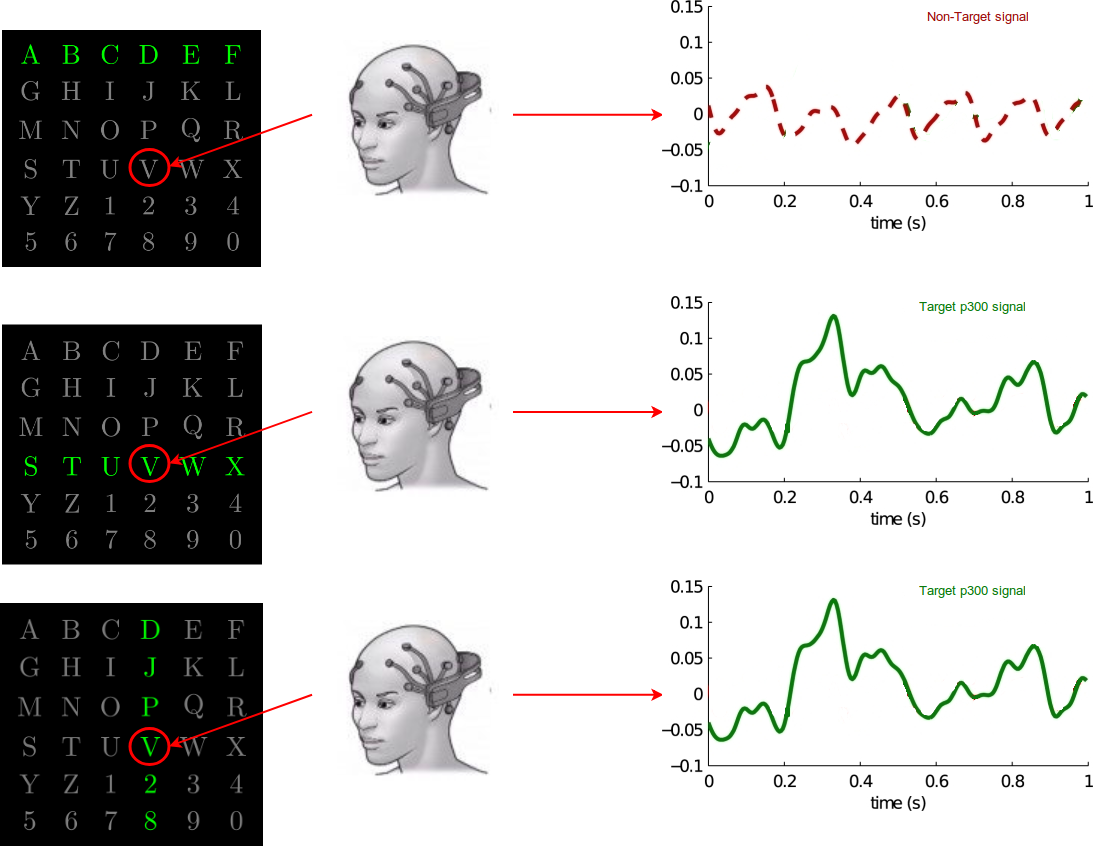
\includegraphics[scale=0.3]{{ImagesSSVEP/p300_speller}.png}}
        \captionsetup{singlelinecheck = false, justification=justified} % used for left alignment
        \caption{Παράδειγμα διέπαφης βασισμένης στα P300 σήματα, για την υλοποίηση μηχανής συλλαβισμού. Ο χρήστης συγκεντρώνεται στο επιθυμητό γράμμα (V), και παράγονται P300 σήματα, όταν φωτιστεί η γραμμή και η στήλη που το περιέχουν.}
        \label{fig:p300_speller}
      \end{figure}

    \subsubsection{Εξωγενή ΠΔ - SSVEP}  
      \paragraph{Περιγραφή} ~\\
      \par Συνήθως τα εξωγενή προκλητά δυναμικά παράγονται από ένα διακριτό ερέθισμα, απομονομένο χρονικά από άλλα πιθανά ερεθίσματα. Ωστόσο, είναι δυνατή η παραγωγή δυναμικών στον εγκέφαλο, προκαλούμενα απο μια ακολουθία διεγέρσεων, οι οποίες εμφανίζονται διαδοχικά με σταθερή συχνότητα. Επειδή η απόκριση σε μια τέτοια ακολουθία οπτικών διεγέρσεων είναι σχετικά σταθερή σε πλάτος, φάση, και συχνότητα, ονομάστηκαν από τον Regan \cite{Regan1966-gn} οπτικά προκλητά δυναμικά σταθερής κατάστασης, ή αλλιώς Steady State Visual Evoked Potentials (SSVEP). Ωστόσο η ανακάλυψη αυτών των δυναμικών φαίνεται να έγινε πρώτη φορά απο τους Adrian και Matthews \cite{1935-sw}, χωρίς όμως να τους δώσουν κάποια συγκεκριμένη ονομασία. 
      \par Η σημαντική λεπτομέρεια που καθιστά τα SSVEP τόσο χρήσιμα στην υλοποίηση διεπαφών εγκεφάλου - υπολογιστή, είναι πως η συχνότητα της προκαλούμενης κυματομορφής στον εγκέφαλο, συμπίπτει με την συχνότητα των οπτικών παλμών της διέγερσης. Με αυτόν τον τρόπο, δημιουργώντας οπτικές πηγές που εκπέμπουν παλμούς σε διαφορετικές συχνότητες, μπορούμε να αντιστοιχίσουμε κάποιες επιθυμητές εντολές σε κάθε μία από αυτές, και συνεπώς μέσω ανάλυσης των παραγώμενων SSVEP σημάτων, να ανιχνεύεται η φωτεινή πηγή στην οποία είναι συγκεντρωμένος ο χρήστης, δηλαδή η εντολή την οποία θέλει να πραγματοποιήσει.  

      \par Το σημείο του εγκεφάλου που παράγονται τα SSVEP σήματα βρίσκεται στον ινιακό φλοιό (occipital lobe), το οποίο είναι λογικό αν σκεφτούμε πως εκέι βρίσκεται το κέντρο επεξεργασίας της όρασης στον εγκέφαλο. Στο απλό σύστημα 10-20 υπάρχουν μόνο δύο ηλεκτρόδια που καλύπτουν τον φλοιό, τα  Ο1 και Ο2, ένω στις επαυξημένες εκδοχές του συστήματος, βρίσκουμε επιπλέον και τα ηλεκτρόδια, Oz που βρίσκεται ανάμεσα στα Ο1 και Ο2, καθώς και τα PO3, PO7, POz, P04, P08, που καλύπτουν τα σύνορα μεταξύ ινιακού και βρεγματικού λοβού. Στις περισσότερες μελέτες χρησιμοποιείται διάφοροι πιθανόι συνδυασμοί των παραπάνω ηλεκτροδίων, η και όλα. Ωστόσο η καλύτερη ποιότητα SSVEP σήματος, φαίνεται να εμφανίζεται στα O2 και Oz \cite{Oikonomou2016-te}.
    \begin{figure}[H]
        \centering
        \noindent\makebox[\textwidth]{\includegraphics[scale=0.1]{{ImagesSSVEP/occ_electrodes}.png}}
        \captionsetup{singlelinecheck = false, justification=justified} % used for left alignment
        \caption{Ηλεκτρόδια που καλύπτουν τον ινιακό λοβό και την γύρω περιοχή.}
        \label{fig:occ_electrodes}
    \end{figure}
    
    
% ΠΟΙΕΣ ΣΥΧΝΟΤΗΤΕΣ, 
      
      %ΔΗΜΟΓΡΑΦΙΚΑ ΠΟΙΟΙ ΜΠΟΡΟΥΝ
      %ΕΠΗΡΕΑΖΕΤΑΙ ΑΠΟ ΠΟΛΛΕΣ ΠΑΡΑΜΕΤΡΟΥΣ 
        χρωμα, οπτικη διεγερση, ψυχολογικη κατασταση, επιπεδα φωτος περιβαλλοντος
      \paragraph{Οπτική Διέγερση} ~\\
      \label{subsec:visual_stimulus}  
      \par Ίσως ο πιο σημαντικός παράγοντας κατά την υλοποίηση της διεπαφής, και ένα από αυτά που επηρεάζουν πιο πολύ την ποιότητα του σήματος,  είναι ο τρόπος με τον οποίο θα επιτευχθεί η επαναλαμβανόμενη διέγερση στον αμφιβληστροειδή χιτώνα, προκειμένου να παραχθούν SSVEP σήματα στον ινιακό λοβό του εγκεφάλου. Κάνοντας μια ανασκόπηση στην βιβλιογραφία παρατηρούμε πως υπάρχουν δύο βασικοί τρόποι επίτευξης της επαναλαμβανόμενης οπτικής διέγερσης (ΕΟΔ) : α) Χρησιμοποιώντας εναλλασσόμενα μοτίβα που παράγονται σε οθόνες (συνήθως LCD) και β) Κάνοντας χρήση πηγών φωτός που αναβοσβήνουν
    
    \begin{figure}
    \centering     %%% not \center
    \subfigure[Figure A]{\label{fig:a}\includegraphics[width=60mm]{{{ImagesSSVEP/occ_electrodes}.png}}}
    \subfigure[Figure B]{\label{fig:b}\includegraphics[width=60mm]{{{ImagesSSVEP/occ_electrodes}.png}}}
    \caption{my caption}
    \end{figure}
    

\end{document}
